\chapter{Event reconstruction}\label{chap:Rec}
\minitoc
The raw detector infromation could not be used in the physics analysis. It is required to have a separate process of interpretation of electronics signals, called reconstruction. It is used to determine the particles, born in the collision, their momentia, direction and vertexes, they are coming from. In this chapter the reconstruction and indentification of the objects at \atlas experiment, used in the analysis will be described. 

It should be noted, that the missing transverse energy reconstruction stands separately, since the standard procedure was not applicable for 2.76 TeV data and a different approach have been adapted.

\section{Tracks and vertexes}
The tracks are reconstructed from the ID infromation. The reconstruction can be divided into 2 steps. 
On the first step the inside-out algoritm is used for the pixel and silicon detector. Tracks are reconstructed from the random 3-points seed in the detector and then adds the new points, while moving to the interaction point using the the Kalman filter.  The Kalman filter is the iterative algorithm that provides the best estimate based on projection of previous and current measurment.  Abiguities in the track candidates are resolved and tracks are extended in TRT.

At the second step, algorithm searches for the segments, reconstructed in TRT and then extends them into the silicon detector. The tracks in TRT with no silicon extension are referred as TRT-standalone tracks. 

Vertexes are reconstucted using the iterative vertex finding algorithm. The vertex starts from the z-position at the beamline of one of the tracks. The \chiD fit is performed on that seed and nearby tracks. The tracks, that are displaced for more, than 7$\sigma$ are treated as a separate vertex. The procedure is repeated till no new vertexes are found. During the reconstruction vertexes are required to contain at leas 2 tracks, but the requirement of the 3 tracks could give more robustness. From the vertex candidates, the vertex with highest sum of the transverse momenta of the outgoing tracks is defined as a primary vertex.

\section{Electron reconstruction and identification}

Due to the detector design electrons are divided into the 2 groups: central and forward. For the central electrons ($| \eta |$ < 2.5 ) there is a tracking information available. Presence of the ID track allows to perform the precise reconstruction and identification. On another hand, for the forward  ($| \eta |$ > 2.5 ) electrons could be reconstructed using just the calorimeter information, so the different algorithm is used. In this section the identification of the central electrons and reconstruction for both central and forward electrons will be discussed.

\subsection{Central electrons reconstruction}
The central electron reconstruction starts from the clusters in the EM calorimeter. On the first step the calorimeter is divided by the grid with the cell size $\Delta \eta \times \Delta \phi = 0.25 \times 0.25$. The EM calorimeter clusters are formed from the cells with total transverse energy in all layers above 2.5 GeV using the sliding window algorithm with size $3\times5$ cells. The position of the cluster is determined from its barycenter.

On the second step track with $P_{T}$ > 0.5 GeV are extrapolated to the middle layer of the EM calorimeter. A track and a cluster are considered mathched to each other if the distance between track and cluster is $|\Delta\eta|$ < 0.5 GeV. In order to take into account effect of the bremsstrahlung losses the azimutal distance is allowed within $\Delta\phi$ < 0.1 on the side where the extrapolated track bends as it traverses the solenoidal magnetic field.

An electron is considered to be reconstructed if at least 1 track is matched to EM cluster. In case if there are several tracks passing the requirements, the tracks with silicon hits are given the priority, an the match with the smallest distance $\Delta R = \sqrt{\Delta\eta^2+\Delta\phi^2}$. In case if there is no track matched, the cluster is treated as a photon candidate.

After the track matching the cluster size is optimised. The cluster size is enlarged to $3\times7$ and $5\times5$ in barrel and end-cap EM respectively. The total reconstructed electron energy is determined from the corrected cluster energy, estimated energy deposit in the material in front of EM and the estimated energy deposits outside of the cluster and calorimeter. The absolute energy scale determination is described in Sec.\ref{}
\subsection{Forward electrons reconstruction}
Since there is no tracking in the forward region (2.5 < $|\eta|$ < 4.9), the electron could be reconstructed using just the information from EMEC and FCAL detectors. Opposite to the central electrons with fixed size of the cell, for forward electrons the topological clustering algorithm is used \cite{Lampl:1099735}. The main principle of this algorithm is that cells with energy higher than expected noise, are merged together iterativelly. The average noise in the cell is obtained in the calibration runs and includes a contribution from pile-up. The cluster tarts from the cell with significant energy and then expanded by neighborhood cells. If 2 clusters are sharing 1 neighborhood cell, they are merged together. The threshold, defined as $t=\frac{E_{cell}}{E_{noise}}$, is 4 and 2 for the starting the cell and expanding neighborhood respectively. 

The energy of the electrons is defined as the sum of the energies, taking into account for energy losses in passive material in front of calorimeter. The direction of the electron is defined as the barycentre of the cluster cells.
\subsection{Electron identification}

The application of additional criteria on reconstructed electrons allows to get better purity of the sample and exlude objects, that can be misidentified as electrons, such as: jets and electrons from the photon conversion. 

The identification of the central electron is based on a sequential cuts,  on calorimeter infromation, tracking and combined variables. There are 3 sets of selection criteria, used for a physics analyses, designed in hierarchical way at to provide incriased background rejection with cost of decreasing identification efficiency. They are:
\begin{description}
\item[Loose] The loose identification criteria  uses the shower shape variables in first and second layer of EM calorimeter and the fraction of energy, deposited in hadronic calorimeter. There are also additional requirements on electron track and track-cluster matching.
\item [Medium] The medium selection is made out of loose identification with adding the information from the 3-rd level of EM calorimeter, transverse impact parameter $d_0$ and TRT (to recject charged hadron background) if avaliable. Additionaly the measured hit in the innermost layer of pixel is reuired to discriminate against the photon conversions. These requirements are allowing to increase the background-rejection power by an order of magnitude, compared to loose.
\item [Tight] The tight selection uses the full information of the particle identification tools avaliable. In addition to medium criteria, it puts stricter requirements on track quality, on ration of EM cluster energy to the track momentum and veto on reconstructed photon conversion vertices assosiated with the cluster. The overall strength of background rejection is 2 times higher, that for a medium selection.
\end{description}

It should be noted, that neither of these criteria requires no additional tracks close to the identified electrons. The optimization of these requirements (called isolation requirements) is left for the dedicated analysis. 

\section{Muon reconstruction and identification}\label{sec:MuonRec}

The \atlas experiment uses the information from ID and muon spectrometer  for a precise reconstruction of the muons. Energy measurments in calorimeter can also be used for the muon identification. The muons, based on the information, avaliable from these detectors, can be divided into different types:
\begin{description}
\item[Combined (CB)] Muons with track both in ID and MS, that could be matched to each other. This is the main type of the muons.
\item[Segment-tagged (ST)] Muons with track in the ID and at least one local track segment in the MDT or CSC chambers. This type of muons could be used for the small $P_{T}$ muons or in the reduced MS acceptance region.
\item[Stand-Alone (SA)] These are the muons, that are crossing at least 2 layers of MS chambers, but have no reconstucted track in the ID. The parameters of the track are determined using the extrapolation to the primary vertex, taking into account the estimated energy loss in the detector in front of MS. These muons are mainly used to extend the acceptance up to $|\eta|$<2.7, where there is no ID information.
\item[Calorimeter-tagged (CaloTag)]  Muons, that have a track in the calorimeter, that can be associated with the minimum ionizing particle.
\end{description}

The muons are reconstructed in MS in two steps: first the local segments within one layer are combined and then the segments are combined combined in a full track. The reconstruction of the MS and combined ID-MS track can be done using one of the two independent reconstruction procedures \cite{AtlasPerf}, called Staco and Muid.  

The Muid algorithm performes full track refit using the parameters from ID and MS\cite{Muid}. 
For the staco algorithm the reconstruction of the track in MS starts from the segment from the outers station. The segments from middle and  inner layers are iterativelly added till the full track is obtained. The matching between ID and MS sub-detectors performed via statistical combination of the parameters in ID and MS using the corresponding covariance matrices\cite{Staco}. Staco algorithm is the algorithm, used in this analysis. 

The following additional requirements are applied on ID track for the muons:
\begin{itemize}
\item  at least 1 pixel hit
\item at least 2 SCT hits
\item at most 2 active pixel or SCT hits, that are transversed by the track, but have no hit.
\item in the region of full TRT acceptance (0.1 < $|\eta|$ < 1.9) at least 9 TRT hits.
\end{itemize}


\section{Missing transverse energy reconstruction}\label{sec:EtMissRec}
\atlas detector has almost 4$\pi$ coverage. This allows to calculate imbalance of energies inside calorimeter, especially transversal part of it called \etmiss.  In W-analyses \etmiss is used as a proxy for neutrino from a $W \to l\nu$ decay. It leaves detector without interacting with it and that causes large energy imbalance in an eventA. In this section two methods of \etmiss reconstruction and the reasons for using non-standard one will be discussed.

\subsection{Standard missing transverse energy reconstruction}

\begin{figure}[!tb]
\begin{minipage}[h]{0.49\linewidth}
\center{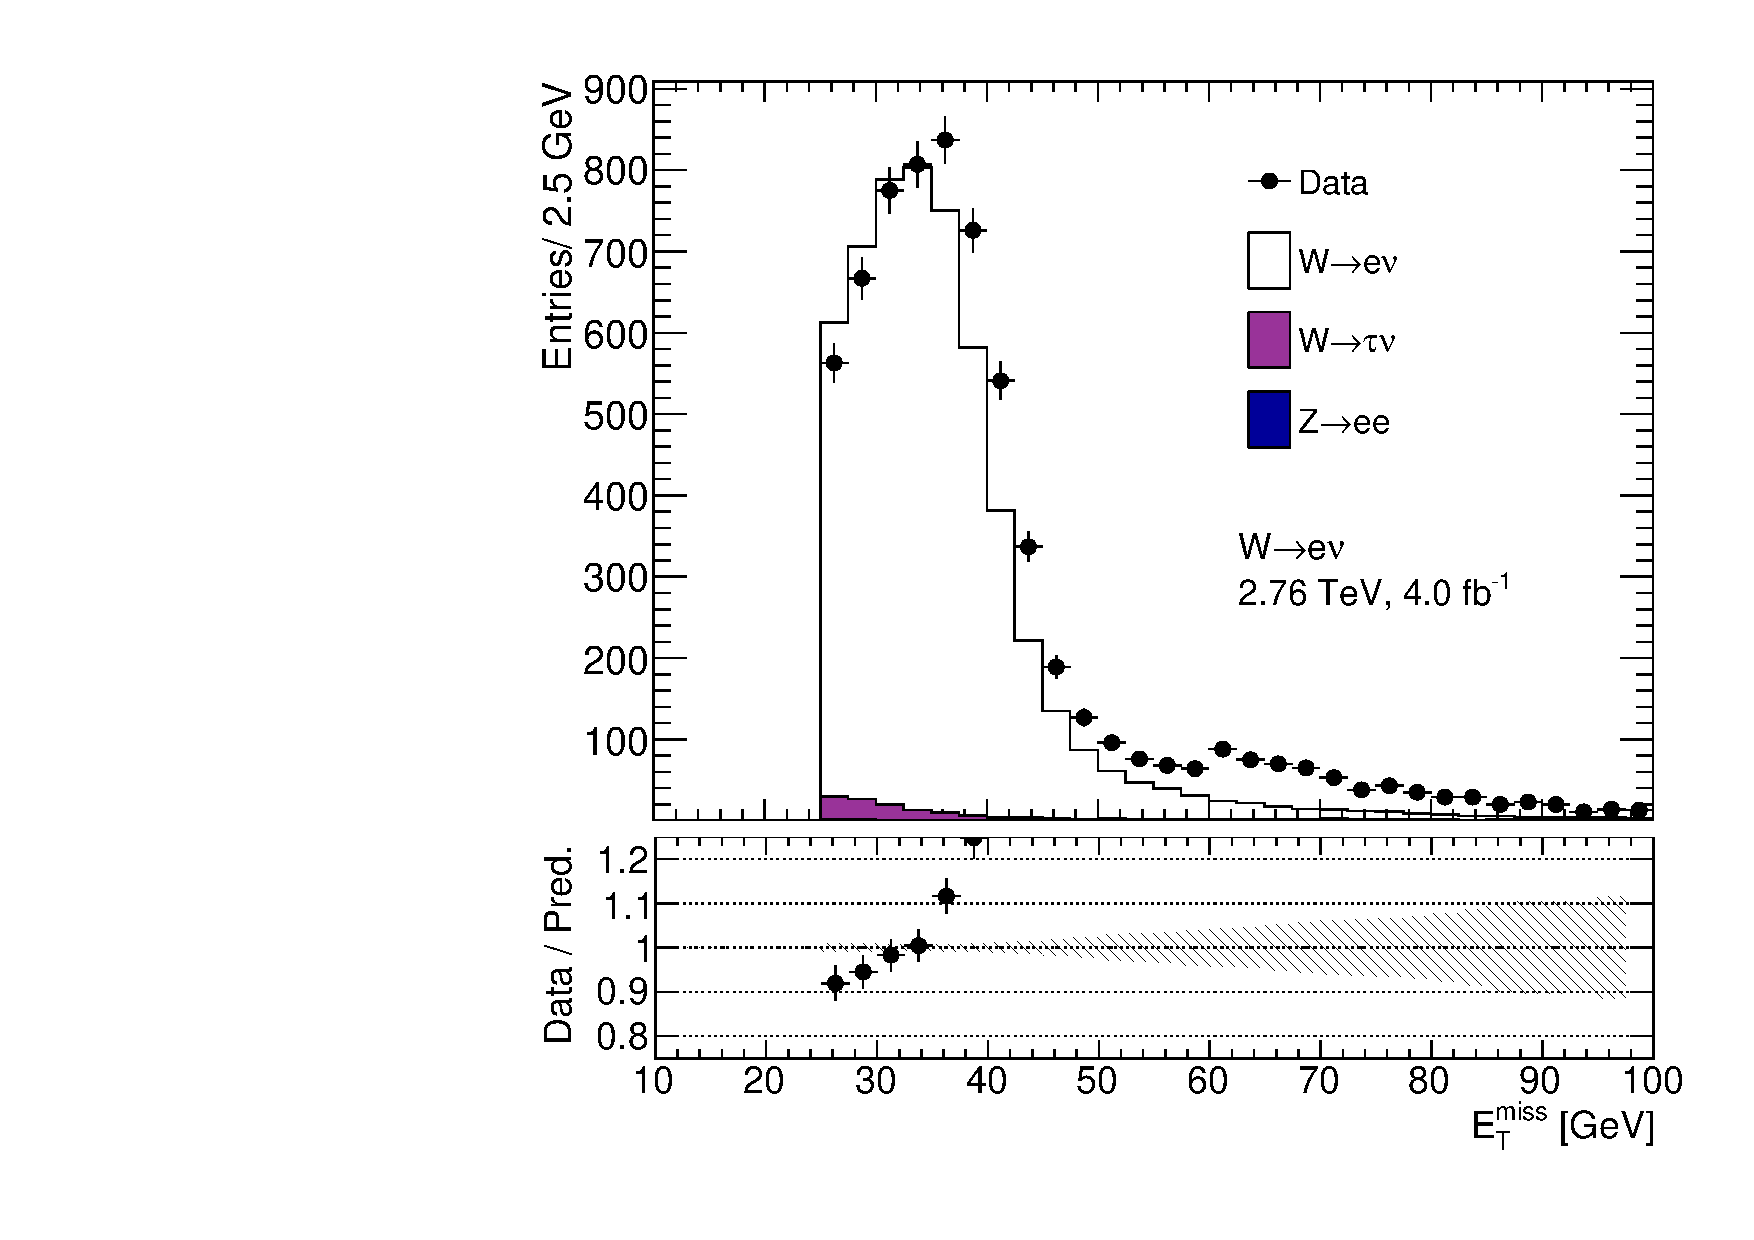
\includegraphics[width=1.\linewidth]{HadronRecoil/WenuRefFinal.pdf} \\ a)}
\end{minipage}
\hfill
\begin{minipage}[h]{0.49\linewidth}
\center{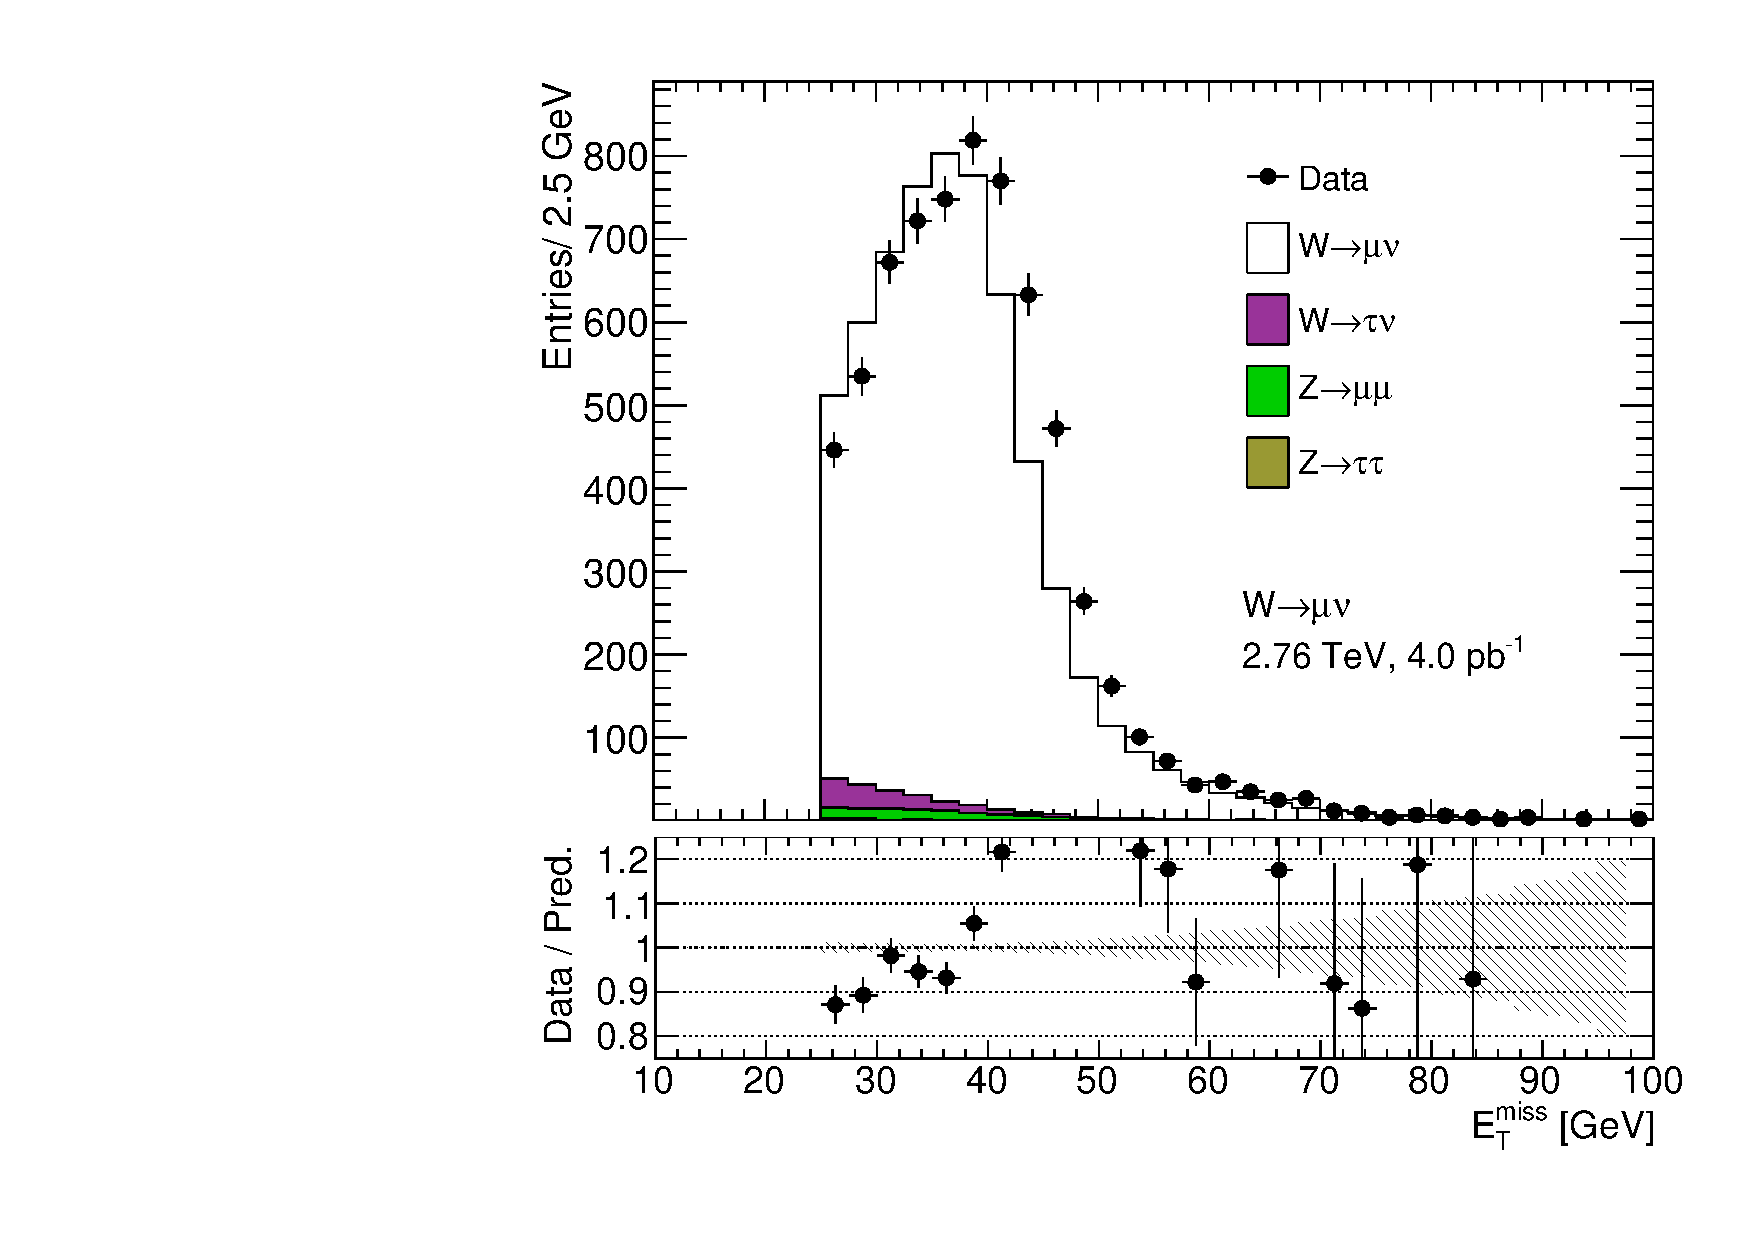
\includegraphics[width=1.\linewidth]{HadronRecoil/WmunuRefFinal.pdf} \\ b)}
\end{minipage}
\caption{Missing transverse energy distribution for a) the \wenu selection and  b) the \wmunu selection from Chap. \ref{chap:EventSelection}. \etmiss  calculated using the standard \atlas algorithm. The expected contributions from all backgrounds are estimated with Monte Carlo simulations, except for QCD background that is not included. All Monte-Carlo corrections from Chap. ~\ref{chap:MCCor} are applied. There are visible discrepancies between data and MC, that cannot be explained by the contribution of the QCD background, which is expected mainly in the low \etmiss region (Sec. \ref{sec:QCD}).}
\label{ris:EtMissRefFinal}
\end{figure}

Standard reconstruction of \etmiss at \atlas experiment \cite{Aad2012} uses transverse energy deposits in the calorimeter, energy losses in cryostat and reconstructed muons for a calculation:
\begin{equation}
E_{x(y)}^{miss} = E_{x(y)}^{miss, calo} +  E_{x(y)}^{miss, cryo} +  E_{x(y)}^{miss, muon}.
\end{equation}

The calorimeter term is using information from reconstructed physics objects for calibration of the cell response. The total transverse energy in calorimeter is defined as:
\begin{equation}
E_{x(y)}^{miss} = E_{x(y)}^{miss, e} + E_{x(y)}^{miss, \gamma} + E_{x(y)}^{miss, \tau} + E_{x(y)}^{miss, jets} + E_{x(y)}^{miss,SoftTerm} + E_{x(y)}^{miss, \mu}.
\end{equation}
where each term is calculated as a negative sum of the calibrated reconstructed objects, projected onto the x and y directions. Each jet with energy $P_T$>20 GeV is corrected for a pile-up and a jet energy scale is applied. Soft term is calculated from topoclusters and tracks, that are not assosiated with high-pt objects. To avoid double counting, muon energy loss  in the calorimeter is  subtracted from \etmiss.  The \etmiss muon term is calculated from the momenta of muons measured in a range of pseudorapidity $| \eta | < 2.7 $. Since pileup has a significant effect on the \etmiss performance several methods of pileup suppression are used \cite{ATLAS-CONF-2014-019}.

The runs at 2.76 TeV are characterized by a low pileup (mean number of interaction per bunch crossing < 1.0), so the usage of a procedure optimized for high pileup 8 TeV runs may not be optimal. It was examined and found out, that there are big discrepancies between the \etmiss distributions for data and MC simulation, as shown in Fig. ~\ref{ris:EtMissRefFinal}, where the missing transverse energy for data is compared to signal and background MC predictions. 

The differences are visible in both electron and muon channels and cannot be explained by the (missing on the control plots) contribution from the QCD background, which is expected mainly in the low \etmiss region (see Sec. \ref{sec:QCD}). 



\subsection{Reconstruction of missing transverse energy from hadronic recoil}


\begin{figure}[!tbp]
\begin{center}
\begin{minipage}[h]{0.49\linewidth}
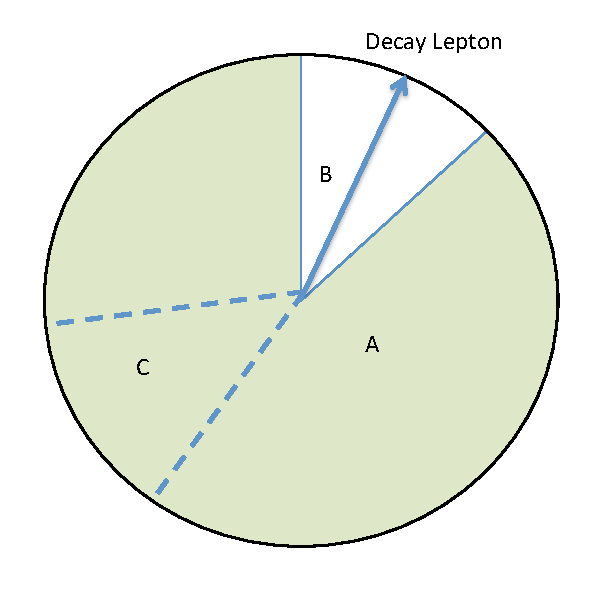
\includegraphics[width=1\textwidth]{HadronRecoil/ReplacementCluster.pdf}
\end{minipage}

\caption{Definition of different zones in the calculation of the cluster-based hadronic recoil. Zone B is excluded from hadronic recoil calculation because it contains decay lepton. To describe properly the overall acitivity it is replaced by the zone C, rotated in the direction of B. Zone A corresponds to the rest of the calorimeter\cite{HRPlots}.}
\label{ris:subsCone}
\end{center}
\end{figure}

A different way of \etmiss calculation  was developed for W and Z decays by the W mass measurements group \cite{HadrRecoilFirst}. This procedure is based on a requirement of a balance in the transverse momentum of a W-boson and the initial (quark-gluon) state radiation:
\begin{equation}
\vec{P}_{T}^{W} = \vec{P}_T^l+\vec{P}_T^{\nu}= \sum{\vec{P}_{T}^{ISRquarks,gluon}}, 
\end{equation}
where $\sum{\vec{P}_{T}^{ISRquarks,gluon}}$ is a transverse momentum of partons from the initial state radiation, also called hadronic recoil (HR), $\vec{P}_T^l$ and $\vec{P}_T^{\nu}$ are the transverse momenta of lepton and neutrino respectively. Therefore, \etmiss can be determined as:
\begin{equation}
E_{T}^{miss} = - P_T^{\nu} =  - HR + \ptl
\end{equation} 

This procedure assumes, that recoil arises from one single leading jet, and the rest  is coming from a soft hadronic activity. The hadronic recoil is computed as a vector sum of calorimeter clusters:
\begin{equation}
HR= \sum_{i=0}^{N_{topo}}\vec{p}_T^{topo}
\end{equation}
while a scalar sum of all transverse energy contributions corresponds to the hadronic activity in the event:
\begin{equation}\label{eq:sumet}
\sum E_T =\sum_{i=0}^{N_{topo}} E_T^{topo}
\end{equation}
To avoid double counting of lepton energy losses in the calorimeter, the clusters inside a cone with a radius $dR$ = 0.2 around the lepton direction are excluded from this calculation.To compensate for the subtracted soft activity from the cone, a replacement cone is added (Fig. \ref{ris:subsCone}). This cone is defined as a cone at the same pesudorapidity, but at a different $\phi$. It should be far from any other lepton and hadronic recoil direction. The cone is then rotated to the original lepton direction. This definition does not take into account the jet reconstruction aspects.   

Fig. \ref{ris:HadrRecoilEtMiss} shows the control plots for the distributions of missing transverse energy calculated using the hadronic recoil procedure. In both electron and muon channels the agreement between data and MC simulation is much better than in the case of the standard procedure described in a previous chapter. It was desided to use hadronic recoil \etmiss reconstruction method in 2.76 TeV data analysis.


\begin{figure}[!tbp]
\begin{minipage}[h]{0.49\linewidth}
\center{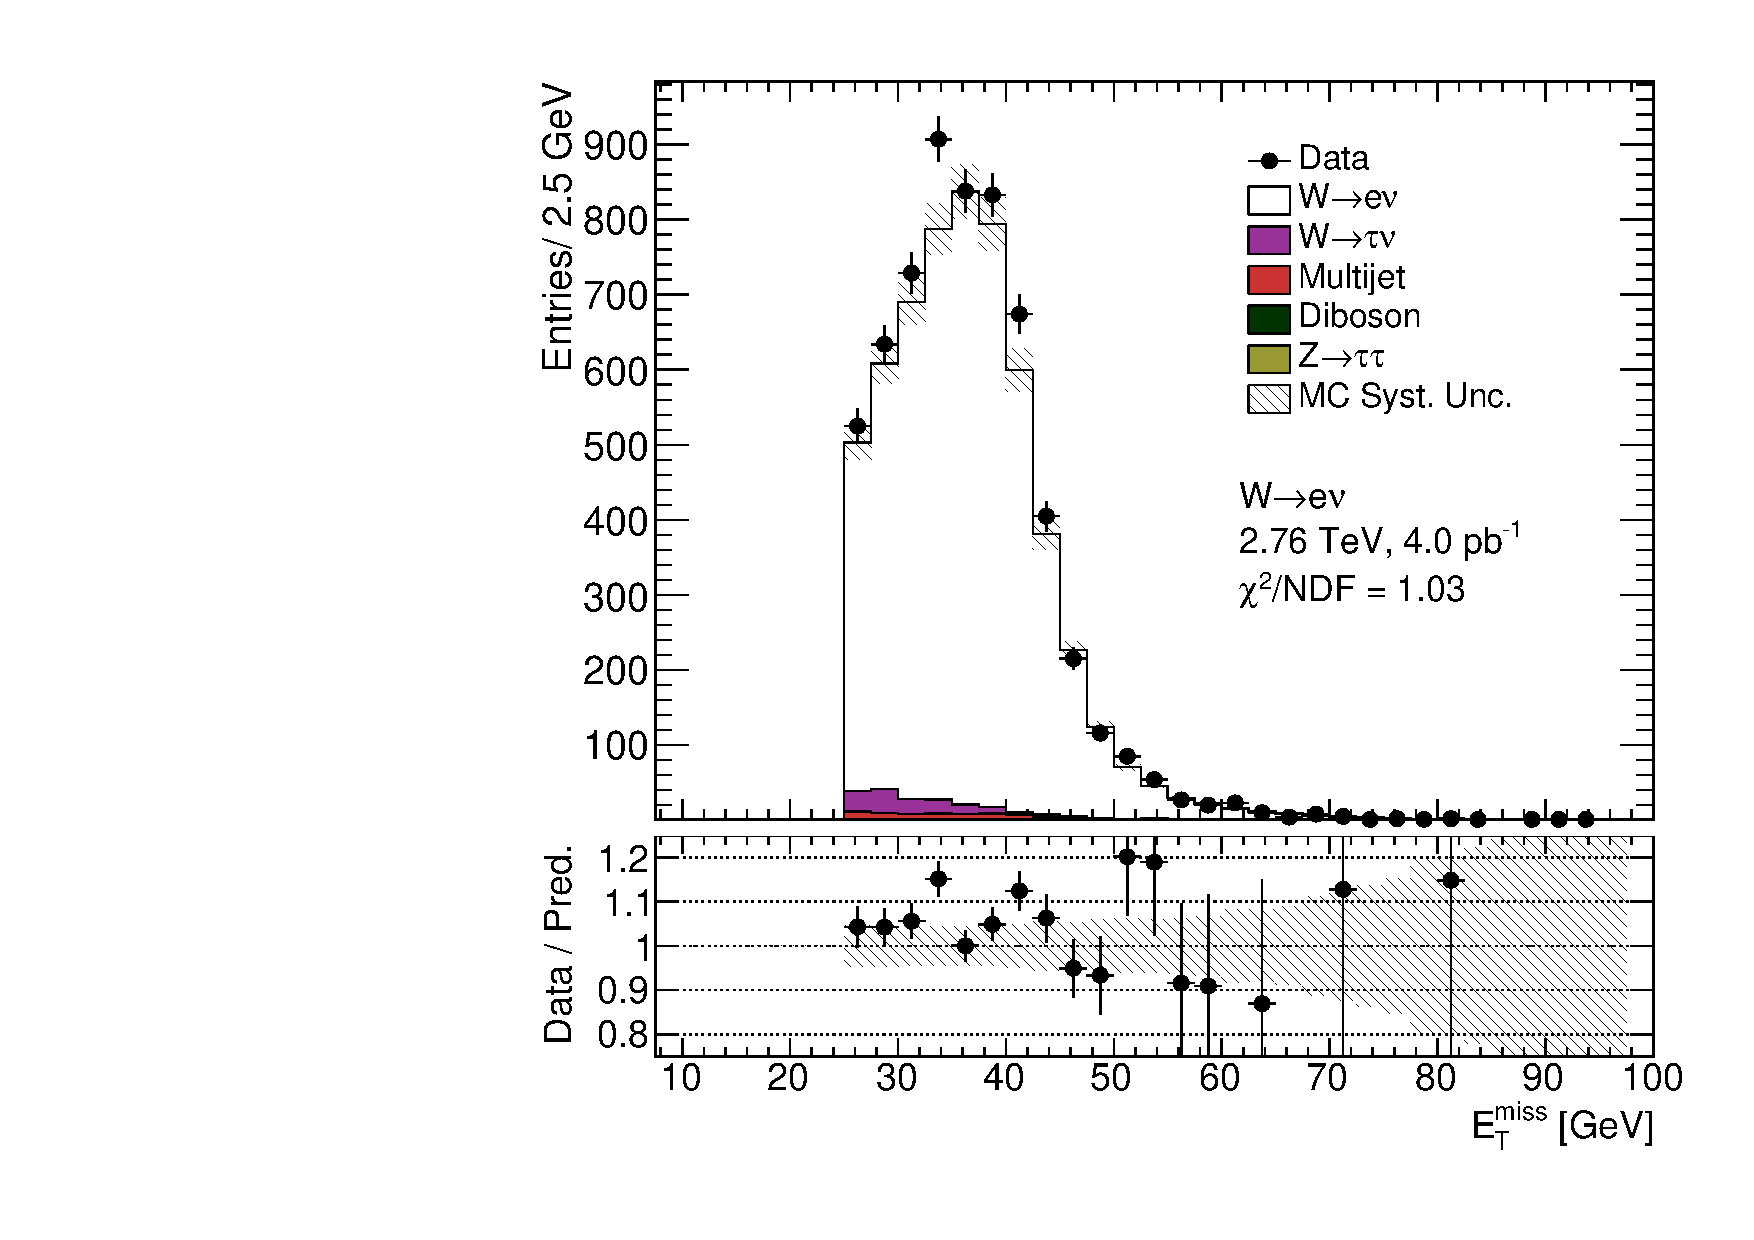
\includegraphics[width=1.\linewidth]{HadronRecoil/W_Boson_etMiss.pdf} \\ a)}
\end{minipage}
\hfill
\begin{minipage}[h]{0.49\linewidth}
\center{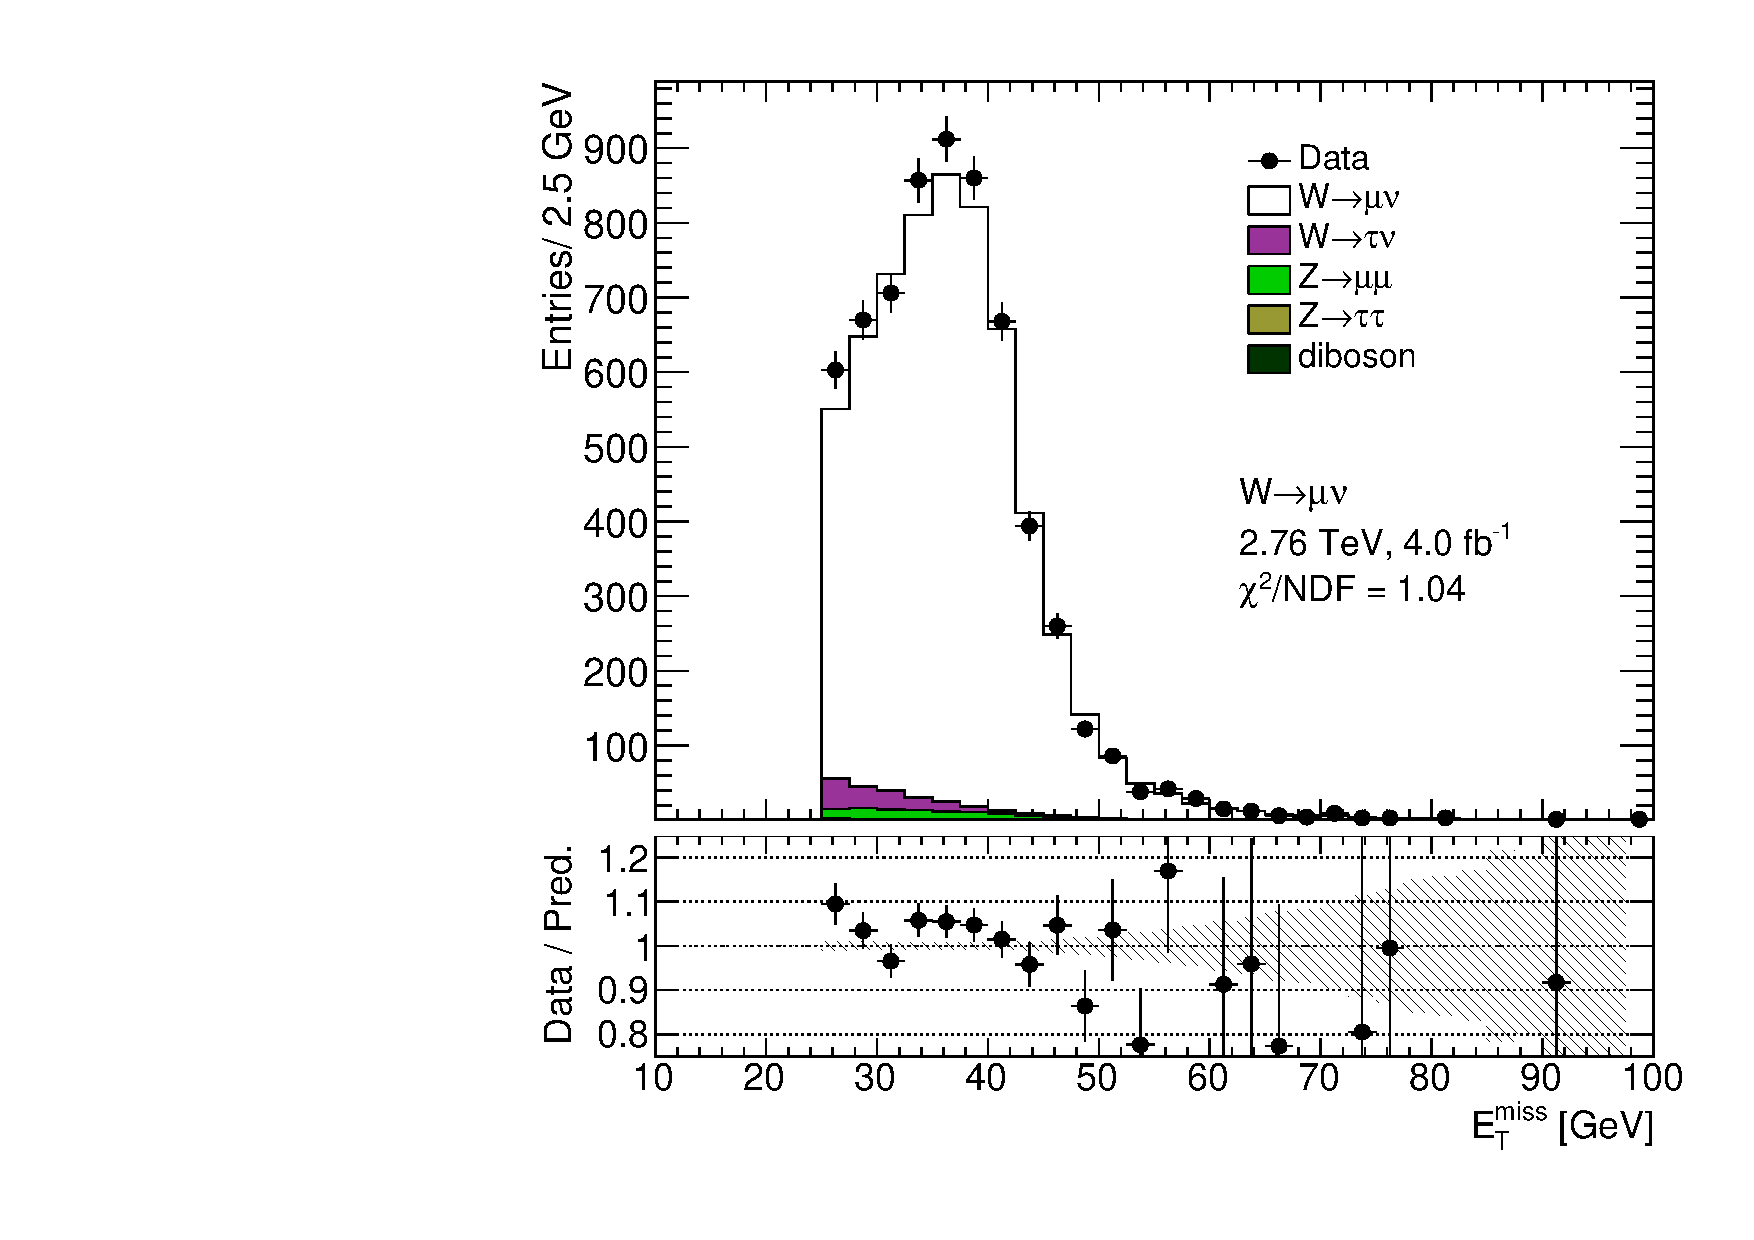
\includegraphics[width=1.\linewidth]{HadronRecoil/Wmu_Boson_etMiss.pdf} \\ b)}
\end{minipage}
\caption{Missing transverse energy distribution for a) the \wenu selection and  b) the \wmunu selection from Chap. \ref{chap:EventSelection}. \etmiss  calculated using the hadronic recoil algorithm. The expected contributions from all backgrounds are estimated with Monte Carlo simulations, except for QCD background that is not included. All Monte-Carlo corrections from Chap. ~\ref{chap:MCCor} are applied.}
\label{ris:HadrRecoilEtMiss}
\end{figure}


